%!TEX root = ../Project.tex

\subsection{Allocation algorithm}

% Writeup from the meeting with JC

% [@todo nice and modular]
% [@todo list constraints mathematically]

\subsubsection{Human aspects}
\label{sec:algo_humanaspects}

During the research period, discussions with academic and administrative staff
in both pilot departments revealed that the current method of module
allocation is not particularly complex. With several hundred students in the
History department, it is impossible for a human to do a uniformly ``fair''
job of allocating modules to students. The staff simply try their best to
allocate as many high choices as possible.

With this information in hand, a score function was designed for the
constrained optimisation problem that also kept the module allocation system
as simple as possible.

One could imagine an imaginary score function that a staff member might have
in their head while allocating modules:

\begin{itemize}
  \item A first choice is perfect -- if every student received every one of
        their first choices, they would be happy.
  \item A second or third choice is alright -- a student would not be too
        displeased to be taking their second or third choice.
  \item A fourth or fifth choice should be avoided if possible, but is not a
        show-stopper.
  \item One would expect a student who was being made to take their sixth or
        lower choice to be fairly unhappy.
\end{itemize}

Mathematically, one could sum a score for each student as follows:

$$
1(x_1) + 5(x_2) + 30(x_3) ...
$$

...where $x_i$ is the number of $i^{th}$ choices that that student was
allocated. The constant applied to the $i^{th}$ choice indicates a penalty
applied by the system -- this penalty increases depending on how negative that
choice is deemed to be.

While not particularly complex, one would expect that minimising this score
function would maximise the number of highly ranked choices.

Eliciting these ideas explicitly from the pilot departments was one of the
harder parts of interacting with the project clients, and in fact the final
coefficients used were not confirmed until a project group meeting on 23
February, just two weeks before the allocation was due to be performed.

The Archaeology department commented that they could not recall ever having to
give a student their fourth choice or below, as they are a fairly small
department (with less than 3\% \textbf{@todo CHECK this!} of all York
undergraduates). This ensures that they normally have sufficient capacity to
offer every student their first, second or rarely third choice.

The History department is far larger than Archaeology, and additionally
reserves a number of spaces on their modules for visiting students. This will
place a strain on the allocation, as the department anticipates there will
most likely not be enough space on the most popular modules for every student
that wants to take them. History aim to give their students ``two from five''
-- that is to say, for a student ranking a group of eight modules, the two
that they will take were among their top five choices.

The final coefficients used in the objective function are shown in
Figure~\ref{gurobi_coeff}.

The hard constraints on the optimisation problem are as follows:

\begin{itemize}
  \item The lower cap on a module (a module will not run if with less than the
        required number of students)
  \item The upper cap on a module (a staff member is not able to provide a
        certain quality of teaching to more than the maximum number of
        students)
  \item The number of credits a student must take from a particular group of
        modules (each student must have exactly the same workload as their
        peers)
\end{itemize}

The following constraints will be loaded into a constrained optimisation
solver and an allocation will be generated.

\subsubsection{Pseudocode}

The binary variables in this system are every student along with every module
that they can be allocated. They are written as $x_{Student,Module}$.

This block of pseudocode ensures that the hard constraint is met such that
each module has a number of students allocated greater than the minimum number
but lower than the cap.

\algsetup{indent=2em}
\begin{algorithmic}
\FORALL{Module in Modules}
  \STATE $min(Module) \leq \displaystyle\sum_{Students}x_{Student,Module} \leq cap(Module)$
\ENDFOR
\end{algorithmic}

This block ensures each student is allocated the correct number of credits.

\begin{algorithmic}
\FORALL{Student in Students}
  \FORALL{Group in Groups}
    \STATE $\displaystyle\sum_{Module \in Group \cap ok(Student)} credit(Module) = credit'(Group) - elective(Group,Student)$
  \ENDFOR
\ENDFOR
\end{algorithmic}

And the objective function that the solver will attempt to maximise is:

$$\displaystyle\sum_{Student, Module} rank'(Student, Module)x_{Student, Module}$$

...where a rank of 1 might return a coefficient of, say, 4000.

\subsubsection{Gurobi}

[@todo update graph with new points]

% Generated using R:
% points <- c(2048, 1000, 480, 235, 120, 60, 30, 15, 6, 2, 1, 1, 0, 0, 0)
% plot(points, xlab="Rank of module", ylab="Coefficient", main="Graph of coefficient against module ranks")
% lines(points)
% dev.copy(pdf, '/path/to/gurobi_coefficients.pdf')
% dev.off()

\begin{figure}
  \begin{center}
    \fbox{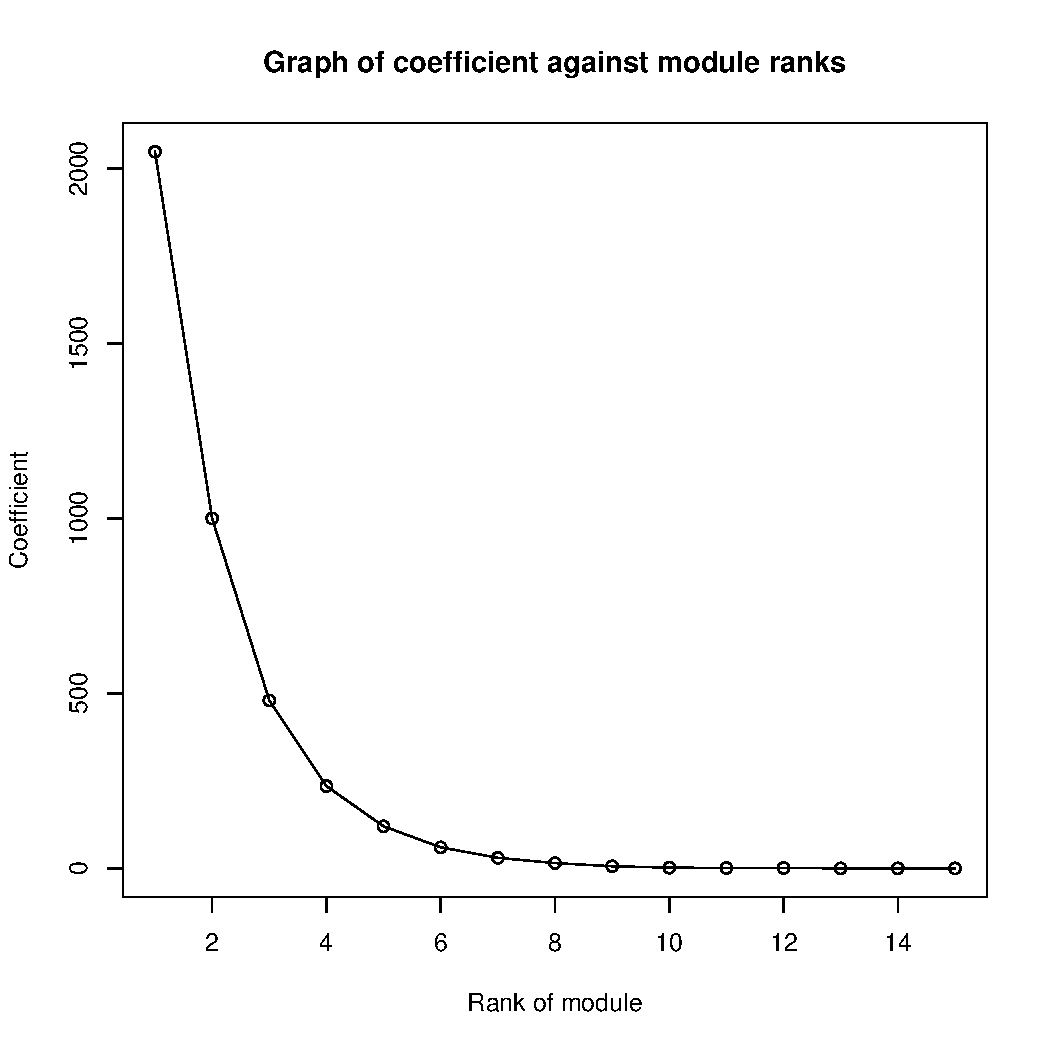
\includegraphics[width=0.6\linewidth]{images/gurobi_coefficients.pdf}}
  \end{center}
  \caption{Coefficients used with Gurobi}
  \label{gurobi_coeff}
\end{figure}

Figure~\ref{gurobi_coeff} shows a graph of the coefficients that were used
with Gurobi. It demonstrates that the information provided to the solver
approximates the imaginary score function a staff member might use.

To begin with, the Gurobi Python interface was used to prototype the model.
Once the Gurobi solver was working correctly on static data using the Python
interface, it was transferred to the application and switched to using the
Java interface.

As the project implementer is more familiar with Python than with Java, it was
faster to prototype using the Python interface. Additionally, there is less
development overhead required with Python (i.e. no compilation necessary). A
copy of the Python prototype is included in
Appendix~\ref{sec:gurobipythonprototype}.
